\documentclass[tikz,border=10pt]{standalone}
\begin{document}
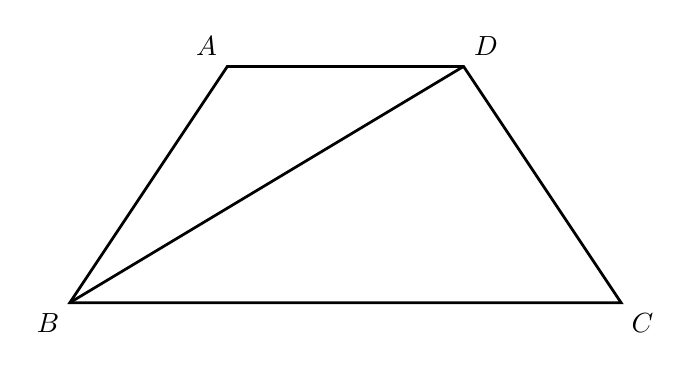
\begin{tikzpicture}[line width=1pt]
\coordinate (A) at (2,3);
\coordinate (B) at (0,0);
\coordinate (C) at (7,0);
\coordinate (D) at (5,3);
\draw (A) -- (B) -- (C) -- (D) -- cycle;
\draw (B) -- (D);
\node[above left] at (A) {$A$};
\node[below left] at (B) {$B$};
\node[below right] at (C) {$C$};
\node[above right] at (D) {$D$};
\end{tikzpicture}
\end{document}
